\chapter{Error estimation}
\label{ch:errorprop}

Suppose that the extinction of the dinosaurs has been dated at 65 Ma
in one field location, and a meteorite impact has been dated at 64 Ma
elsewhere.  These two numbers are effectively meaningless in the
absence of an estimate of precision. Taken at face value, the dates
imply that the meteorite impact took place 1 million years after the
mass extinction, which rules out a causal relationship between the two
events. However, if the analytical uncertainty of the age estimates is
significantly greater than 1 Myr, then such of a causal relationship
remains plausible. There are two aspects of analytical uncertainty that
need to be considered:

\begin{itemize}
  \item{\bf accuracy} is the closeness of a statistical estimate to
    its true (but unknown) value.
  \item{\bf precision} is the closeness of multiple measurements to
    each other.
\end{itemize}

\noindent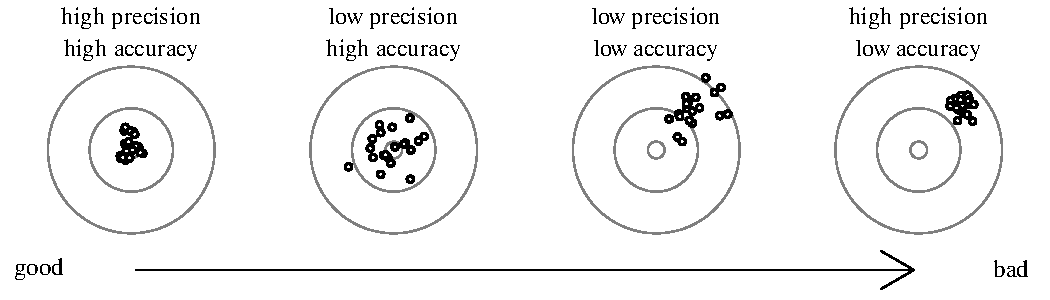
\includegraphics[width=\textwidth]{../figures/accuracyvsprecision.pdf}
\begingroup \captionof{figure}{Darts board illustration of accuracy
  (closeness to the centre) and precision (closeness of the
  measurements). The best case scenario combines high precision with
  high accuracy. The worst case scenario combines high precision with
  low accuracy. This is the worst possible situation because the high
  precision gives false confidence in the data.\medskip}
\label{fig:darts}
\endgroup

Accuracy can be assessed by analysing \emph{reference materials} (or
`secondary standards') whose true parameter values are known through
independent means. This procedure involves little statistics and won't
be discussed further in this chapter. Quantifying precision is a more
involved process that is also known as \textbf{error
  propagation}. This procedure will be discussed in some detail in the
following sections.

\section{Error propagation}
\label{sec:linearerrorprop}

Suppose that physical quantity ($z$) is calculated as a function ($g$)
of some measurements ($x$):
\begin{equation}
z = g(x)
\label{eq:zgx}
\end{equation}

\noindent and suppose that replicate measurements of $x$ ($x_i$, for
$i=1...n$) \emph{follow a normal distribution} with mean $\bar{x}$ and
standard deviation $s[x]$. Then these values can be used to estimate
$s[z]$, the standard deviation of the calculated value $z$.  If the
function $g$ is (approximately) linear in the vicinity of $\bar{x}$,
then small deviations $(\bar{x}-x_i)$ of the measured parameter $x_i$
from the mean value $\bar{x}$ are proporational to small deviations
$(\bar{z}-z_i)$ of the estimated quantity $z$ from the mean value
$\bar{z}=g(\overline{x})$.\medskip

Recall the definition of the sample standard deviation and variance
(Equation~\ref{eq:stdevrepeat}):
\begin{equation}
s[z]^2 \equiv \frac{1}{n-1} \sum_{i=1}^{n} (z_i-\bar{z})^2
\label{eq:varz}
\end{equation}

Let $\partial{z}/\partial{x}$ be the slope of the function $g$ with
respect to the measurements $x$ (evaluated at $\bar{x}$)\footnote{In
  this chapter, all derivatives will be evaluated at the measured
  value.} then:
\begin{equation}
(z_i-\bar{z}) \approx \frac{\partial z}{\partial x} (x_i-\bar{x})
\label{eq:zi-z}
\end{equation}

\noindent\begin{minipage}[t][][b]{.45\textwidth}
  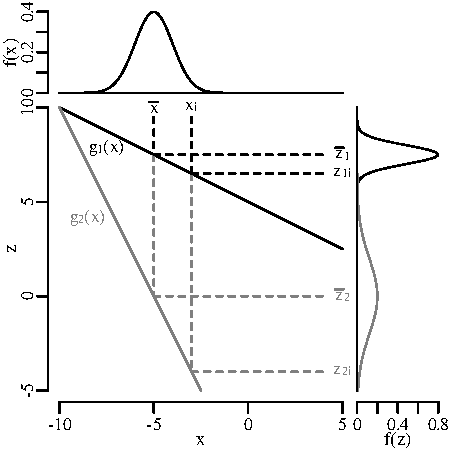
\includegraphics[width=\textwidth]{../figures/errorprop2d.pdf}\medskip
\end{minipage}
\begin{minipage}[t][][t]{.55\textwidth}
\captionof{figure}{Error propagation of two linear functions, $g_1$
  (black line) and $g_2$ (grey line). The input data $\{x_i\}$ are
  normally distributed around some average value $\bar{x}$. Error
  propagation estimates the dispersion of the inferred quantity $z_i$
  from the dispersion of the measurements $x_i$.  Deviations
  $(x_i-\bar{x})$ from the average $x$-value are reduced (for function
  $g_1$) or magnified (for function $g_2$) depending on the slope of
  the functions, resulting in deviations of the dependent variable
  that are smaller $(z_{i1}-\bar{z}_1)$ or greater
  $(z_{i2}-\bar{z}_i)$ than $(x_i-\bar{x})$.  }
  \label{fig:errorprop2d}
\end{minipage}

Plugging Equation \ref{eq:zi-z} into \ref{eq:varz}, we obtain:
\begin{equation}
  \begin{split}
    s[z]^2 & \approx \frac{1}{n-1} \sum_{i=1}^{n}
    \left[(x_i-\overline{x}) \frac{\partial z}{\partial x}\right]^2 \\
    & = \left[\frac{\partial z}{\partial x}\right]^2 \left[\frac{1}{n-1}
      \sum_{i=1}^{n} (x_i-\overline{x})^2 \right] 
      = \left[\frac{\partial z}{\partial x}\right]^2 s[x]^2\\
    \Rightarrow s[z] & = \left|\frac{\partial z}{\partial x}\right| s[x]
  \end{split}
  \label{eq:errorprop1d}
\end{equation}

$s[z]$ is the \textbf{standard error} of $z$, i.e.  the
\textit{estimated} standard deviation of the inferred quantity $z$.\medskip

Equation~\ref{eq:errorprop1d} is the general equation for the
propagation of uncertainty with one variable.  Next, let us move on to
multivariate problems. Suppose that the our estimated quantity ($z$)
is calculated as a function ($g$) of two measurements ($x$ and $y$):
\begin{equation}
z = g(x,y)
\label{eq:zfxy}
\end{equation}

\noindent and further suppose that $x$ and $y$ follow a bivariate
normal distribution (Equation~\ref{eq:2dgauss}), then $\mu_x$,
$\mu_{y}$, $\sigma_{x}$, $\sigma_{y}$ and $\sigma_{x,y}$ can all be
estimated (as $\bar{x}, \bar{y}, s[x], s[y]$ and $s[x,y]$) from the
input data ($\{x_i, y_i\}$, for $i~=~1...n$). These values can then be
used to infer $s[z]$, the standard error of $z$, in exactly the same
way as for the one dimensional case.\medskip

Differentiating $g$ with respect to $x$ and $y$:
\begin{equation}
  z_i - \overline{z} \approx (x_i-\overline{x}) \frac{\partial z}{\partial x} +
  (y_i-\overline{y}) \frac{\partial z}{\partial y}
  \label{eq:dg}
\end{equation}

Plugging Equation~\ref{eq:dg} into Equation~\ref{eq:varz}:
\begin{equation}
  s[z]^2 \approx \frac{1}{n-1} \sum_{i=1}^{n} \left[
    (x_i-\overline{x}) \frac{\partial z}{\partial x} +
    (y_i-\overline{y}) \frac{\partial z}{\partial y} \right]^2
\end{equation}

After some rearranging (similar the derivation of
Equation~\ref{eq:errorprop1d}), this leads to:
\begin{equation}
  s[z]^2 \approx s[x]^2 \left(\frac{\partial z}{\partial x}\right)^2 +
  s[y]^2 \left(\frac{\partial z}{\partial y}\right)^2 +
  2~s[x,y] \frac{\partial z}{\partial x} \frac{\partial z}{\partial y}
  \label{eq:errorprop2d}
\end{equation}

This is the general equation for the propagation of uncertainty with
two variables, which can also be written in a matrix form:
\begin{equation}
s[z]^2 \approx
\left[
  \begin{array}{@{}cc@{}}
\frac{\partial z}{\partial x} & \frac{\partial z}{\partial y}
\end{array}
\right]
\left[
\begin{array}{@{}cc@{}}
s[x]^2 & s[x,y]\\
s[x,y] & s[y]^2
\end{array}
\right]
\left[
\begin{array}{@{}c@{}}
\frac{\partial z}{\partial x} \\
\frac{\partial z}{\partial y}
\end{array}
\right]
\label{eq:errorprop2dmatrix}
\end{equation}

where the innermost matrix is known as the \emph{variance-covariance}
matrix and the outermost matrix (and its transpose) as the
\emph{Jacobian matrix}. The advantage of the matrix formulation is
that it can easily be scaled up to three or more dimensions.

\noindent\begin{minipage}[t][][b]{.55\textwidth}
  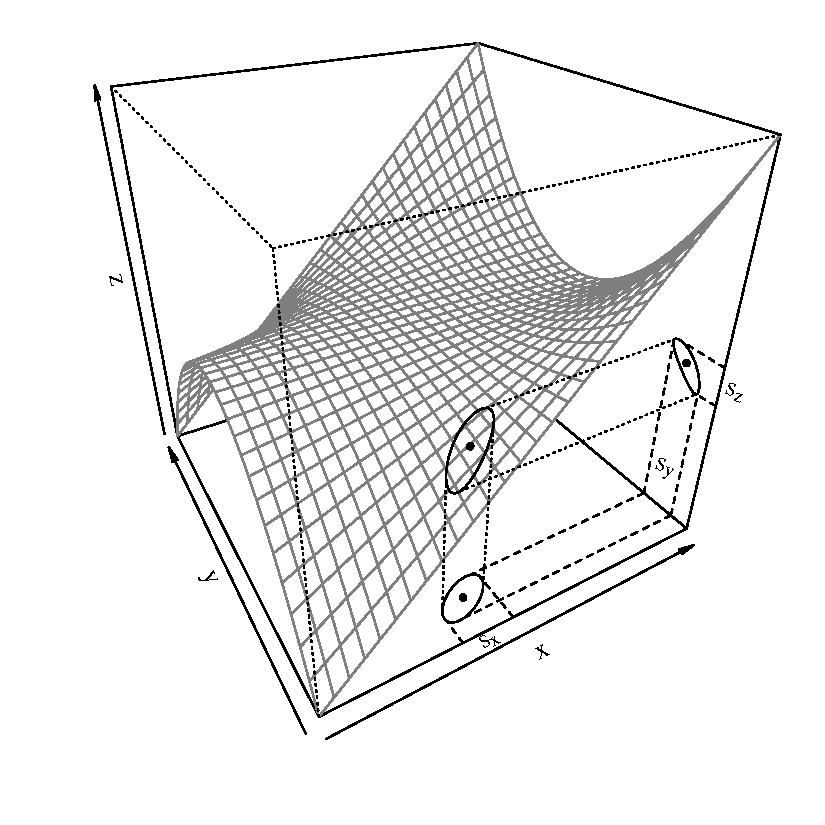
\includegraphics[width=\textwidth]{../figures/errorprop3d.pdf}\medskip
\end{minipage}
\begin{minipage}[t][][t]{.45\textwidth}
  \captionof{figure}{Error propagation of a bivariate function $z =
    g(x,y)$. The uncertainty in $z$ is \emph{approximately}
    proportional to the slope of the surface $g$ w.r.t. the
    measurements $x$ and $y$. If the curvature of the 3D surface is
    minor relative to the uncertainties, then said surface can be
    \emph{locally} approximated by a plane. Using such a linear
    approximation, the size of the error ellipses ($s[x]$, $s[y]$)
    around the mean measurements (black dots) linearly scales with
    corresponding deviations in the inferred quantity ($s[z]$).}
  \label{fig:errorprop3d}
\end{minipage}

\section{Examples}
\label{sec:errorpropexamples}

Equation~\ref{eq:errorprop2d}/\ref{eq:errorprop2dmatrix} is the
generic error propagation formula. This section will apply this
formula to some common mathematical functions. It will use the
following notation:

\begin{itemize}
\item{$a, b, c, \ldots$} are constants, i.e. values that are known
  without uncertainty ($s[a]=s[b]=s[c]=0$);
\item{$x$ and $y$} are measurements whose uncertainties ($s[x]$ and
  $s[y]$) were estimated from replicates;
\item{$z = g(x,y)$} is the estimated quantity.
\end{itemize}

\noindent For example, $z = x/2 + y^3$ can be written as $z = a x +
y^b$, where $a=1/2$ and $b=3$.

\begin{enumerate}
  
\item{\bf addition:}
  \[
  z = a + b x + c y
  \]

  Taking the derivatives of $z$ with respect to $x$ and $y$:
  
  \[
  \frac{\partial z}{\partial x} = b \mbox{~and~} \frac{\partial z}{\partial y} = c
  \]

  Plugging these into Equation~\ref{eq:errorprop2d}:
  \begin{equation}
    s[z]^2 = b^2 s[x]^2 + c^2 s[y]^2 + 2bc~s[x,y]
    \label{eq:addition}
  \end{equation}

  If $x$ and $y$ are uncorrelated (i.e., $s[x,y]=0$), then the
  variance of the sum equals the sum of the variances.

\item{\bf subtraction:}
  \[
  z = a x - b y
  \]

  The partial derivatives of $z$ with respect to $x$ and $y$ are

  \[
  \frac{\partial z}{\partial x} = a \mbox{~and~}
  \frac{\partial z}{\partial y} = -b
  \]

  Plugging these into Equation~\ref{eq:errorprop2d}:
  \begin{equation}
    s[z]^2 = a^2 s[x]^2 + b^2 s[y]^2 - 2ab~s[x,y]
    \label{eq:subtraction}
  \end{equation}

  Note that, if $x$ and $y$ are uncorrelated, then
  Equations~\ref{eq:addition} and \ref{eq:subtraction} are identical.

\item{\bf multiplication:}
  \[
  z = a x y
  \]

  The partial derivatives are
  \[
  \frac{\partial z}{\partial x} = a y \mbox{~and~}
  \frac{\partial z}{\partial y} = a x
  \]

  Plugging these into Equation~\ref{eq:errorprop2d}:
  \[
  s[z]^2 = (a y)^2 s[x]^2 + (a x)^2 s[y]^2 + 2(a y)(a x)~s[x,y]
  \]

  Dividing both sides of this equation by $z^2 = (a x y)^2$:
  \[
  \left(\frac{s[z]}{z}\right)^2 =
  \left(\frac{a y}{a x y} s[x]\right)^2 +
  \left(\frac{a x}{a x y} s[y]\right)^2 +
  2\left(\frac{a y}{a x y}\right)\left(\frac{a x}{a x y}\right) s[x,y]
  \]

  which simplifies to:
  \begin{equation}
    \left(\frac{s[z]}{z}\right)^2 = \left(\frac{s[x]}{x}\right)^2 +
    \left(\frac{s[y]}{y}\right)^2 + 2 \frac{s[x,y]}{x y}
    \label{eq:multiplication}
  \end{equation}

  $(s[x]/x)$ and $(s[y]/y)$ represent the \textit{relative standard
    deviation}s of $x$ and $y$. These are also known as the
  \textbf{coefficient}s \textbf{of variation} (CoV).  If $x$ and $y$
  are uncorrelated, then the squared CoVs of a product equals the sum
  of the squared CoVs.

\item{\bf division:}
  \[
  z = a \frac{x}{y}
  \]

  The partial derivatives are
  \[
  \frac{\partial z}{\partial x} = \frac{a}{y} \mbox{~and~}
  \frac{\partial z}{\partial y} = -\frac{a x}{y^2}
  \]

  Plugging these into Equation~\ref{eq:errorprop2d}:
  \[
  s[z]^2 = \left(\frac{a}{y}\right)^2 s[x]^2 +
  \left(-\frac{a x}{y^2}\right)^2 s[y]^2 +
  2\left(\frac{a}{y}\right)\left(-\frac{a x}{y^2}\right) s[x,y]
  \]

  Dividing both sides of this equation by $z^2 =
  \left(a x / y\right)^2$:
  \[
  s[z]^2 = \left(\frac{a}{y}\frac{y}{ax}\right)^2 s[x]^2 +
  \left(-\frac{a x}{y^2}\frac{y}{ax}\right)^2 s[y]^2 +
  2\left(\frac{a}{y}\frac{y}{ax}\right)
  \left(-\frac{a x}{y^2}\frac{y}{ax}\right) s[x,y]
  \]

  which simplifies to:
  \begin{equation}
    \left(\frac{s[z]}{z}\right)^2 = \left(\frac{s[x]}{x}\right)^2 +
    \left(\frac{s[y]}{y}\right)^2 - 2 \frac{s[x,y]}{x y}
    \label{eq:division}
  \end{equation}

  If $x$ and $y$ are uncorrelated, then the uncertainty of the
  quotient (Equation~\ref{eq:division}) equals the uncertainty of the
  product (Equation~\ref{eq:multiplication}).

\item{\bf exponentiation:}
  \[
  z = a e^{bx}
  \]

  The partial derivative of $z$ w.r.t. $x$ is
  \[
  \frac{\partial z}{\partial x} = ab e^{bx}
  \]

  Plugging this into Equation~\ref{eq:errorprop2d}:
  \[
  s[z]^2 = \left(ab e^{bx}\right)^2 s[x]^2
  \]

  Dividing both sides by $z^2 = \left(a e^{bx}\right)^2$:
  \[
  \left(\frac{s[z]}{z}\right)^2 =
  \left(\frac{ab e^{bx}}{a e^{bx}}s[x]\right)^2 
  \]

  which simplifies to
  \begin{equation}
    \left(\frac{s[z]}{z}\right)^2 = b^2 s[x]^2
    \label{eq:exponentiation}
  \end{equation}

\item{\bf logarithms:}
  \[
  z = a \ln[bx]
  \]

  The partial derivative of $z$ w.r.t. $x$ is
  \[
  \frac{\partial z}{\partial x} = \frac{a}{x}
  \]

  Plugging this into Equation~\ref{eq:errorprop2d}:
  \begin{equation}
    s[z]^2 = a^2 \left(\frac{s[x]}{x}\right)^2
    \label{eq:logarithms}
  \end{equation}

\item{\bf power:}
  \[
  z = a x^b
  \]

  The partial derivative of $z$ w.r.t. $x$ is
  \[
  \frac{\partial z}{\partial x} = ab x^{b-1}
  \]

  Plugging this into Equation~\ref{eq:errorprop2d}:
  \[
  s[z]^2 = \left(ab x^{b-1}\right)^2 s[x]^2
  \]

  Dividing both sides by $z = a x^b$:
  \[
  \left(\frac{s[z]}{z}\right)^2 = \left(\frac{ab x^{b-1}}{a x^{b}}s[x]\right)^2 
  \]

  which simplifies to
  \begin{equation}
    \left(\frac{s[z]}{z}\right)^2 = b^2\left(\frac{s[x]}{x}\right)^2
    \label{eq:power}
  \end{equation}

\item{\bf other:}

  Error propagation for more complicated functions can either be derived
  from Equation~\ref{eq:errorprop2d} directly, or can be done with
  Equations~\ref{eq:addition}--\ref{eq:power} using the \textbf{chain
    rule}. For example, consider the following equation:
  \begin{equation}
    d = d_\circ + v_\circ t + g t^2
    \label{eq:newtons2nd}
  \end{equation}

  \noindent which describes the distance $d$ travelled by an object as a
  function of time $t$, where $d_\circ$ is the position at $t=0$,
  $v_\circ$ is the velocity at $t=0$, and $g$ is the acceleration.
  Although Equation~\ref{eq:newtons2nd} does not directly fit into any
  of the formulations that we have derived thus far, it is easy to
  define two new functions that do. Let
  \begin{equation}
    x \equiv d_\circ + v_\circ t
    \label{eq:xvt}
  \end{equation}

  \noindent and
  \begin{equation}
    y \equiv g t^2
    \label{eq:ygt2}
  \end{equation}

  \noindent then Equation~\ref{eq:xvt} matches with the formula for
  addition (Equation~\ref{eq:addition}):
  \[
  z = a + bx + cy
  \]

  \noindent where $a \equiv d_\circ$, $b \equiv v_\circ$, $x \equiv t$,
  $c \equiv 0$ and $y$ is undefined. Then uncertainty propagation of
  Equation~\ref{eq:xvt} using Equation~\ref{eq:addition} gives:
  \begin{equation}
    s[x]^2 = \left(v_\circ s[t]\right)^2
    \label{eq:sx}
  \end{equation}

  Similarly, Equation~\ref{eq:ygt2} matches with the formula for
  powering (Equation~\ref{eq:power}):
  \[
  z = a x^b
  \]

  \noindent where $a \equiv g$, $b \equiv 2$ and $x \equiv t$. Applying
  Equation~\ref{eq:power} to Equation~\ref{eq:ygt2} yields:
  \begin{equation}
    \left(\frac{s[y]}{y}\right)^2 =  2^2 \left(\frac{s[t]}{t}\right)^2
    \Rightarrow s[y]^2 = \left(2 g t^2 \frac{s[t]}{t}\right)^2 =
    \left(2 g t s[t]\right)^2
    \label{eq:sy}
  \end{equation}

  Combining Equations~\ref{eq:xvt} and \ref{eq:ygt2} turns
  Equation~\ref{eq:newtons2nd} into a simple sum:
  \[
  d = x + y
  \]

  \noindent whose uncertainty can be propagated with
  Equation~\ref{eq:addition}:
  \[
  s[d]^2 = s[x]^2 + s[y]^2
  \]

  Substituting Equation~\ref{eq:sx} for $s[x]^2$ and
  Equation~\ref{eq:sy} for $s[y]^2$:
  \[
  s[d]^2 = \left(v_\circ s[t]\right)^2 + \left(2 g t s[t]\right)^2
  \]

  \noindent which leads to the following expression for the
  uncertainty of $d$:
  \begin{equation}
    s[d] = \sqrt{\left(v_\circ s[t]\right)^2 + \left(2 g t s[t]\right)^2}
    \label{eq:sdnewton}
  \end{equation}

  To illustrate the use of this formula, suppose that $d_\circ=0$~m,
  $v_\circ=10$~m/s and $g=9.81$~m/s\textsuperscript{2}.  Further
  suppose that we measure the time $t$ with a watch that has a
  1/10\textsuperscript{th} of a second precision\footnote{Here
    precision refers not to the magnitude of normally distributed
    noise, but to the resolution of the clock.} ($s[t]=0.1$~s). Then
  we can predict how far the object will have travelled after 5
  seconds:
  \begin{equation}
  d = 0 \mbox{~m} +
  10 \frac{\mbox{m}}{\mbox{s}} \times 5 \mbox{~s} +
  9.81\frac{\mbox{m}}{\mbox{s}^2} \times (5 \mbox{~s})^2 = 295.25\mbox{~m}
  \label{eq:snowy}
  \end{equation}

  Using Equation~\ref{eq:sdnewton}, the uncertainty\footnote{Here the
    uncertainty is not a standard error in the traditional sense of
    the word, but we can still use the same error propagation methods
    to compute it.} of $d$ is given by:
  \begin{equation}
  s[d] = \sqrt{\left(10 \frac{\mbox{m}}{\mbox{s}} \times
    0.1\mbox{~s}\right)^2 + 4
    \left(9.81\frac{\mbox{m}}{\mbox{s}^2}\right)^2
    \left(5\mbox{~s}\right)^2\left(0.1\mbox{~s}\right)^2} =
  9.861\mbox{~m}
  \label{eq:haddock}
  \end{equation}

  Thus the predicted displacement after 5~seconds can be reported as
  $295.250\pm{9.861}$~m, or as $295.2\pm{9.9}$~m if we \textbf{round}
  the estimate to two \textbf{significant digits}. Note how
  Equations~\ref{eq:snowy} and \ref{eq:haddock} specifies the units of
  all the variables. Checking that these units are balanced is good
  practice that avoids arithmetic errors.
  
\end{enumerate}

\section{Standard deviation vs. standard error}
\label{sec:stderr}

As defined in Section~\ref{sec:linearerrorprop}, the standard error is
the estimated standard deviation of some derived quantity obtained by
error propagation. The mean of set of numbers is an example of such a
derived quantity, and its estimated uncertainty is called the standard
error of the mean.  Let $\{x_1,x_2, \ldots x_n\}$ be $n$ measurements
of some quantity $x$, and let $\bar{x}$ be its mean
(Equation~\ref{eq:mean}):
\[
\bar{x} = \sum\limits_{i=1}^n \frac{x_i}{n} = \frac{1}{n} \sum\limits_{i=1}^n x_i
\]

Applying the error propagation formula for a sum
(Equation~\ref{eq:addition}):
\[
s[\bar{x}]^2 = \sum\limits_{i=1}^{n}\left(\frac{s[x_i]}{n}\right)^2 =
\left(\frac{1}{n}\right)^2 \sum\limits_{i=1}^{n}s[x_i]^2
\]

If all the $x_i$s were drawn from the same normal distribution with
standard deviation $s[x]$, then
\[
s[\bar{x}]^2 = \left(\frac{1}{n}\right)^2 \sum\limits_{i=1}^{n}s[x]^2 =
n \left(\frac{1}{n}\right)^2 s[x]^2
\]

\noindent which simplifies to
\begin{equation}
  s[\bar{x}] = \frac{s[x]}{\sqrt{n}}
  \label{eq:stderrmean}
\end{equation}

The standard error of the mean monotonically decreases with the square
root of sample size. In other words, we can arbitrarily increase the
\emph{precision} of our analytical data by acquiring more
data. However, it is important to note that the same is generally not
the case for the \emph{accuracy} of those data
(Figure~\ref{fig:darts}). To illustrate the effect of the square root
rule, consider the statistics of human height as an example.  The
distribution of the heights of adult people is approximately normal
with a mean of 165~cm and a standard deviation of 10~cm. There about 5
billion adult humans on the planet. Averaging their heights should
produce a value of 165~cm with a standard error of
$10/\sqrt{5\times{10}^9} = 1.4\times{10}^{-4}$~cm. So even though
there is a lot of dispersion among the heights of humans, the standard
error of the mean is only 1.5 \emph{microns}.

\section{Fisher Information}
\label{sec:FisherInformation}

We used the method of maximum likelihood to estimate the parameters of
the binomial (Section~\ref{sec:binompar}), Poisson
(Section~\ref{sec:poispar}) and normal
(Section~\ref{sec:normalparameters}) distributions. An extension of
the same method can be used to estimate the standard errors of the
parameters without any other information. Let $\hat{z}$ be the maximum
likelihood estimate of some parameter $z$. We can approximate the
log-likelihood with a second order Taylor series in the vicinity of
$\hat{z}$:
\[
  \mathcal{LL}(z) \approx \mathcal{LL}(\hat{z}) +
  \left.\frac{\partial\mathcal{LL}}{\partial{z}}\right|_{\hat{z}}
  \!(z-\hat{z}) +
  \left.\frac{1}{2} \frac{\partial^2\mathcal{LL}}{\partial{z^2}}\right|_{\hat{z}}
  \!(z-\hat{z})^2
\]

By definition, $\partial{\mathcal{LL}}/\partial{z}=0$ at
$\hat{z}$. Therefore, the likelihood ($\mathcal{L}(z) =
\exp[\mathcal{LL}(z)]$) is proportional to:
\[
\mathcal{L}(z) \propto 
\exp\left[
  \frac{1}{2}
  \left.\frac{\partial^2\mathcal{LL}}{\partial{z^2}}\right|_{\hat{z}}
  \!(z-\hat{z})^2
  \right]
\]

\noindent which can also be written as:
\[
\mathcal{L}(z) \propto \exp\!\left[
  -\frac{1}{2} \frac{(z-\hat{z})^2}{
    -\frac{1}{\left.\frac{\partial^2\mathcal{LL}}{\partial{z^2}}\right|_{\hat{z}}}
  }\right]
\]

This equation fits the functional form of the normal distribution
(Equation~\ref{eq:gauss}):
\[
\mathcal{L}(z) \propto \exp\!\left[
  -\frac{1}{2} \frac{(z-\hat{z})^2}{\sigma[z]^2}
  \right]
\]

\noindent which leads to
\begin{equation}
  \hat{\sigma}[z]^2 =
  \frac{1}{-\left.\frac{\partial^2\mathcal{LL}}{\partial{z^2}}\right|_{\hat{z}}}
  \label{eq:Fisher}
\end{equation}

$-\left.\frac{\partial^2\mathcal{LL}}{\partial{z^2}}\right|_{\hat{z}}$ is known as the
\textbf{Fisher Information}. Equation~\ref{eq:Fisher} can be
generalised to multiple dimensions:
\begin{equation}
  \hat{\Sigma} = -\mathcal{H}^{-1}
  \label{eq:multidimFisher}
\end{equation}

\noindent where $\hat{\Sigma}$ is the estimated covariance matrix and
$(\mathcal{H})^{-1}$ is the inverse of the (`Hessian') matrix of
second derivatives of the log-likelihood function with respect to the
parameters.\medskip

To illustrate the usefulness of Equation~\ref{eq:Fisher}, let us apply
it to the Poisson distribution.  Recalling the log-likelihood function
(Equation~\ref{eq:poisLL}) and denoting the maximum likelihood
estimate of the parameter by $\hat{\lambda}$:
\[
\mathcal{LL}(\hat{\lambda}|k) =
k \log[\hat{\lambda}] - \hat{\lambda} - \sum\limits_{i=1}^{k}i
\]

Taking the second derivative of $\mathcal{LL}$ with respect to
$\lambda$:
\begin{equation}
  \left.\frac{\partial^2{\mathcal{LL}}}{\partial{\lambda^2}}\right|_{\hat{\lambda}}\! =
  -\frac{k}{\hat{\lambda}^2}
  \label{eq:d2LLdl2}
\end{equation}

Plugging Equation~\ref{eq:d2LLdl2} into \ref{eq:Fisher}:
\[
  \hat{\sigma}[\lambda]^2 = \frac{\hat{\lambda}^2}{k}
\]

Recalling that $\hat{\lambda} = k$ (Equation~\ref{eq:lambda=k}), we
get:
\begin{equation}
  \hat{\sigma}[\lambda]^2 = \hat{\lambda}
  \label{eq:poisvar}
\end{equation}

Thus we have proven that the variance of a Poisson variable equals its
mean, which was already shown empirically in
Chapter~\ref{ch:poisson}.\medskip

Using the same rationale to estimate the standard error of a binomial
variable, we take the logarithm of Equation~\ref{eq:Lbinom}:
\[
\mathcal{LL}(p|n,k) = \ln\!\binom{n}{k} + k \ln(p) + (n-k) \ln(1-p)
\]

\noindent the second derivative of which is:
\[
\frac{\partial^2\mathcal{LL}}{\partial{p^2}} =
-\frac{k}{p^2} - \frac{n-k}{(1-p)^2}
\]

At the maximum likelihood estimate $\hat{p}=n/k$
(Equation~\ref{eq:phat}), this becomes:
\[
\left.\frac{\partial^2\mathcal{LL}}{\partial{p^2}}\right|_{\hat{p}} =
-\frac{n\hat{p}}{\hat{p}^2} - \frac{n-n\hat{p}}{(1-\hat{p})^2} =
-\frac{n}{\hat{p}(1-\hat{p})}
\]

\noindent so that the variance of $\hat{p}$ is:
\[
s[\hat{p}]^2 = \frac{\hat{p}(1-\hat{p})}{n}
\]

\noindent which proves Equation~\ref{eq:sigmabinom}.
